\documentclass[a4paper,11p]{memoir}

%\pdfoutput=1

\newlength{\figwidth}
% FINAL
%\setlength{\figwidth}{88mm}
% DRAFT
\setlength{\figwidth}{0.65\textwidth}


\usepackage{color}
\definecolor{links}{rgb}{0.7,0,0}   % red
\definecolor{urls}{rgb}{0,0,0.8}    % blue
\definecolor{cites}{rgb}{0,0,0.8}   % blue

\usepackage[colorlinks,hyperindex,linkcolor=links,citecolor=cites,urlcolor=urls]{hyperref} % generates colored links in pdf file
%---------------------------------------------------------
% styles and other macros
\usepackage[nosort]{cite}        
\usepackage{url} 
\usepackage[intlimits]{amsmath}
\usepackage{bbm}
\usepackage{graphicx}
\usepackage{paralist}
\usepackage{verbatim}
\usepackage[stretch=16,shrink=16,step=4]{microtype}
% \usepackage{vmr-symbols-vecbold}
% \usepackage{standard-macros}

\newcommand{\todo}[1]{{\noindent\small\sffamily\slshape\color{red}[#1]}}
\def\matn{\mathcal{N}}

%*******************************************************************************
%!TEX encoding =  

\begin{document}


\title{SPeCTrE\\
Short Packet Communication Toolbox for Wireless Engineers\\[1cm]
Version 0.1}

\author{Contributors (alphabetic order):\\
Giuseppe Durisi, Johan \"Ostman, Yury Polyanskiy, Wei Yang,\dots}


\maketitle

\begin{abstract}

In his 1948 landmark paper, Claude E. Shannon demonstrated that communication with arbitrarily small probability of error is feasible if, and only if, the communication rate is below the so called channel capacity. To achieve this result, codes with large packet size (blocklength) must be employed. 
In the nonasymptotic regime of finite packet size, the interplay between packet error probability, communication rate, and packet size can be described through closed-form achievability and converse bounds.
The SPeCTrE toolbox provides numerical routines to evaluate these bounds for some channel models that occur in wireless communication applications. 
The toolbox is under development and the participation of additional members of the information and communication theory communities in this endevour is warmly welcomed!
\end{abstract}
\newpage
\tableofcontents

\newpage
%%%%%%%%%%%%%%%%%%%%%%%%%
\chapter{Motivation}
%
  In his 1948 landmark paper, Claude E. Shannon demonstrated that communication with arbitrarily small probability of error is feasible if, and only if, the communication rate is below the so called channel capacity. 
  To achieve this result, codes with large packet size (blocklength) must be employed. 
 Shannon's channel capacity has served as a useful guideline to design wireless communication systems.

In some applications, however, a more refined analysis of the interplay between packet-error probability, communication rate, and packet size is required.
  This may occur in emerging applications, such as massive machine-to-machine communication for metering, traffic safety, and telecontrol of industrial plants, together with real-time data transfer to enable remote wireless control (tactile internet), which may require the exchange of short packets, sometimes under stringent latency and reliability constraints.
  
Finite-blocklength information theory, a subfield of information theory that benefitted from seminal contributions from Shannon, Strassen, and Dobrushin, among others, is currently a very active field of research. 
Nonasymptotic achievability and converse bounds on the \emph{maximum coding rate} achievable for a given packet size and packet error probability are now available for several channel models that are relevant for wireless communication systems, such as the AWGN channel, the quasi-static Rayleigh fading channel, and the Rayleigh block-fading channel.
The purpose of this toolbox is to provide numerical routines for the computation of these bounds.
In the next chapters, we provide a bare-bone manual on the routines available in this toolbox.



% subsection contributors (end)
%%%%%%%%%%%%%%%%%%%%%%%%%
\chapter{AWGN channel}


General info:
\begin{itemize}
\item Maintainer: Y. Polyanskiy \url{<yp@mit.edu>}

\item Main references: \cite{PPV08,PPV10eneff}

\item Example: See Fig.~\ref{fig:awgn_example} 

\item Channel model:
	$$ Y_j = X_j + Z_j, \quad j=1,\ldots,n $$
	Noise: $Z_j \sim \matn(0,1)$ iid.\\
	Power constraints: Each codeword $x^n$ satisfies
			$$ \sum_{j=1}^n |x_j|^2 \le n P $$

\item Common input/output arguments:
\begin{enumerate}
\item \verb|P| -- input argument; parameter of the power constraint (so $P=10$ is $SNR=10~dB$).
\item \verb|epsil| -- block probability of block error.
\item \verb|lm| or \verb|Lms| -- output argument; $\log_2 M$, log-size of codebook (base-2 information units). 
\item \verb|n| -- input argument; blocklength.\\
		For slow functions that do not support vectorized arguments.
\item \verb|Ns| -- input argument; vector of blocklengths.
\end{enumerate}
\end{itemize}


\begin{figure}
\centering
\begin{verbatim}
	> plot_v3(10, 0.001, 1, 100:20:1000)
\end{verbatim}
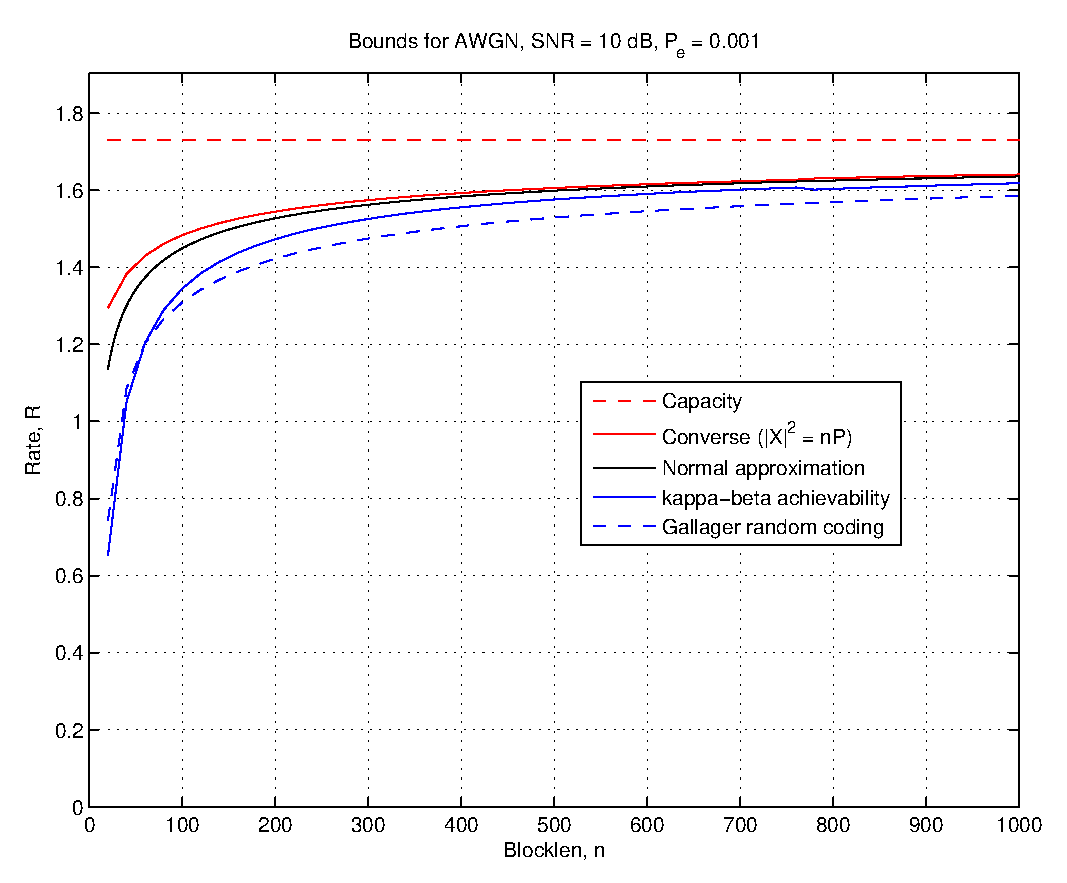
\includegraphics[height=5cm]{plots/awgn_plot3_ex}
\caption{Code and resulting picture for AWGN bounds}\label{fig:awgn_example}
\end{figure}


\section{Summary plot: \texttt{plot\_v3()}}

Definition:
\begin{verbatim}
	function [Ns lb ub feinst gal wlfz] = plot_v3(P, epsil)
\end{verbatim}

This function plots various bounds on the same figure. See Fig.~\ref{fig:awgn_example}.


\section{Achievability: \texttt{shannon\_ach2()}}

Definition:
\begin{verbatim}
	function lm = shannon_ach2(n, epsil, P)
\end{verbatim}

Function computes Shannon's cone-packing achievability bound, see~\cite[(41)]{PPV08}.

\section{Achievability: \texttt{kappabeta\_ach()}}
Format:
\begin{verbatim}
	function Lms = kappabeta_ach(Ns, epsil, P, hack)
\end{verbatim}

This computes the $\kappa\beta$ achievability bound, see left-hand inequality in~\cite[(218)]{PPV08}. If $hack\neq 0$, then we
use asymptotic approximation for $\kappa$. This increases the speed dramatically and is very precise already at $n=10$,
see~\cite[(217)]{PPV08}. If $hack$ is not set, it defaults to $1$.

\section{Achievability: \texttt{gallager\_ach()}}
Format:
\begin{verbatim}
	function lm = gallager_ach(n, epsil, P)
\end{verbatim}

Computes Gallager's achievability bound, see~\cite[(44)]{PPV08}.

\section{Converse: \texttt{converse()}}
Format:
\begin{verbatim}
	function Lms = converse(Ns, epsil, P)
\end{verbatim}

This computes the meta-converse lower bound with $Q_{Y^n} = \matn(0, 1+P)^n$, see right-hand inequality in~\cite[(218)]{PPV08}. 


\section{Normal approximation: \texttt{normapx\_awgn(), normapx\_biawgn()}}

Format:
\begin{verbatim}
	function Lms = normapx_awgn(Ns, epsil, P);
\end{verbatim}

Fast and frequently very precise approximation to both achievability and converse:
	$$ \log M \approx n C - \sqrt{nV} Q^{-1}(\epsilon) + {1\over2} \log n $$


\section{Code database: \texttt{plot\_universe()}}

Code in \verb|universe/plot_universe()| compiles a comparative plot of normalized rate for different codes.
See~\cite[Section IV.D]{PPV08}.


\section{Energy-per-bit bounds}

Format:
\begin{verbatim}
	function En0 = ach_nofb(Lms, epsil);
	function lm = converse_nofb(en0, epsil);
	function lm = normapx_nofb(en0, epsil);
\end{verbatim}

These functions return achievability/converse/normal approximation for the problem of minimal achievable ratio ${E\over
N_0 \cdot \log_2 M}$, where $E$ is the total expended energy over infinite channel uses of AWGN channel with noise
$N_0\over 2$.  These are bounds from~\cite[Theorems 2 and 3]{PPV10eneff}.

%%%%%%%%%%%%%%%%%%%%%%%%%
\chapter{Fading channels}


\section{Rayleigh block-fading channel with no a priori channel state information} % (fold)
\label{sec:rayleigh_block_fading_channel_with_no_channel_state_information}
General info:
\begin{itemize}
  \item Maintainer: G. Durisi \url{<durisi@chalmers.se>}
  
  \item Contributors: G. Durisi, J. \"Ostman, W. Yang

  \item Main reference: \cite{durisi14-12a} 

  \item Example: See Fig. \ref{fig:snr6eps03M2}
  
  \item Channel model:
  
  \item Common input, output arguments: 
  
\end{itemize}
% section rayleigh_block_fading_channel_with_no_channel_state_information (end)

   \begin{figure}[t]
    \centering
      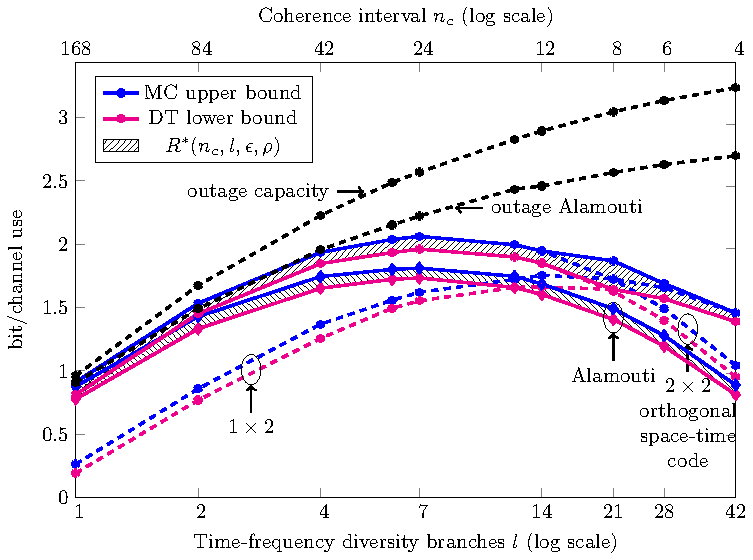
\includegraphics[width=.9\textwidth]{./plots/snr6eps03M2.pdf}
    \caption{Maximum coding rate $R^\ast(n_c,l,\epsilon,\rho)$ for $2\times 2$ MIMO system operating over a Rayleigh block-fading channel with coherence time $n_c$.
    Each packet spans~$l$ coherence intervals. The packet size is $168$ channel uses. The packet error rate is $\epsilon=10^{-3}$.
    The SNR is $\rho=6$ dB.}
    \label{fig:snr6eps03M2}
  \end{figure}
` '
%%%%%%%%%%%%%%%%%%%%%%%%%%%%
\bibliographystyle{IEEEtran}
\bibliography{IEEEabrv,refs}
\end{document}

